\documentclass[9pt,journal,compsoc]{IEEEtran}
\usepackage{amsmath,amssymb,amsbsy}
\usepackage{graphicx}
\usepackage{balance}  % for  \balance command ON LAST PAGE  (only there!)
\usepackage{url}
\usepackage{enumitem}
\usepackage{hyperref}
\usepackage{multirow}
\usepackage{gensymb}
\usepackage{subcaption}
\usepackage[export]{adjustbox}
\usepackage{tabularx, colortbl}
\usepackage{array}
\usepackage{dblfloatfix}
\usepackage{fancyvrb}
\usepackage{gensymb}
\usepackage{listings}
%\usepackage{color,soul}
\usepackage{courier}

\definecolor{codegreen}{rgb}{0,0.6,0}
\definecolor{codegray}{rgb}{0.5,0.5,0.5}
\definecolor{codepurple}{rgb}{0.58,0,0.82}
\definecolor{co_string}{RGB}{95, 135, 0}
\definecolor{co_comment}{RGB}{135, 135, 135}
\definecolor{co_other}{RGB}{135, 95, 175}
\definecolor{co_number}{RGB}{215, 95, 0}
\definecolor{co_keyword}{RGB}{215, 0, 95}
\definecolor{co_special}{RGB}{0, 135, 175}

\lstdefinestyle{custompy}{
    basicstyle=\footnotesize\ttfamily,
    commentstyle=\color{co_comment},
    keywordstyle=\bfseries\color{co_keyword},
    keywordstyle=[2]{\bfseries\color{co_other}},
    stringstyle=\bfseries\color{co_string},
    emphstyle=\bfseries\color{co_special},
    breakatwhitespace=false,
    breaklines=true,
    captionpos=b,
    keepspaces=true,
    showspaces=false,
    showstringspaces=false,
    showtabs=false,
    tabsize=2,
    literate=%
        {0}{{{\color{co_number}0}}}1
        {1}{{{\color{co_number}1}}}1
        {2}{{{\color{co_number}2}}}1
        {3}{{{\color{co_number}3}}}1
        {4}{{{\color{co_number}4}}}1
        {5}{{{\color{co_number}5}}}1
        {6}{{{\color{co_number}6}}}1
        {7}{{{\color{co_number}7}}}1
        {8}{{{\color{co_number}8}}}1
        {9}{{{\color{co_number}9}}}1,
}

\begin{document}
\bstctlcite{IEEEexample:BSTcontrol}

\title{Synopsis: A Distributed Sketch over Voluminous Spatiotemporal Observational Streams}

\author{Thilina~Buddhika, Matthew Malensek, Sangmi Lee Pallickara and Shrideep Pallickara,~\IEEEmembership{Members,~IEEE}%
%\IEEEcompsocitemizethanks{\IEEEcompsocthanksitem T. Buddhika, M. Malensek, S.L. Pallickara and S. Pallickara  are with the Department
%of Computer Science, Colorado State University.
%E-mail: \{thilinab, malensek, sangmi, shrideep\}@cs.colostate.edu\protect}
}

\IEEEtitleabstractindextext{%
\begin{abstract}
    Networked observational devices have proliferated in recent years, contributing to voluminous data streams from a variety of sources and problem domains. These streams often have a spatiotemporal aspect and include multidimensional \emph{features} of interest. Processing such data in an offline fashion using batch systems or data warehouses is costly from both a storage and computational standpoint, and in many situations the insights within the data streams are only useful if they are discovered in a timely manner.

    In this study, we propose \textsc{Synopsis}, a stream processing system that builds a distributed \emph{sketch} of incoming observational data points as they arrive. The sketch summarizes feature values and inter-feature relationships in memory to facilitate real-time query evaluations. As the data streams evolve and user query patterns change, \textsc{Synopsis} can scale up or down appropriately to ensure high accuracy and low query latencies. We evaluate our system in the context of a real-world spatiotemporal dataset and demonstrate its efficacy in both scalability and query evaluations. \\ \\
\end{abstract}

\begin{IEEEkeywords}
data sketches, streaming systems, spatiotemporal data, query evaluations
\end{IEEEkeywords}}
\maketitle

\IEEEdisplaynontitleabstractindextext
\section{Introduction}
\label{sec:introduction}
\cite{buddhika2016neptune}

\subsection{Paper Organization}
The remainder of this paper is organized as follows...


\section{System Overview}
\label{sec:system}
\textsc{Synopsis} is implemented on top of Neptune stream processing system~\cite{buddhika2016neptune} as a specialized layer for geo-spatial data.
In this section, we will briefly introduce Neptune followed by a discussion on the design of \textsc{Synopsis}.

\subsection{Neptune}
Neptune is a distributed stream processing system which is optimized to process high throughput data streams.
It is designed to cope with application requirements such as high volumes of small stream packets, high and variable data rates and heterogeneity within stream processing jobs.
Satisfying these requirements imposes various system level challenges including possible buffer-overflow errors, increased number of context-switches, object creation overhead and memory management issues.
Neptune takes a holistic approach that considers CPU, memory, network and kernel issues to address the above challenges.
This is achieved through employing a set of optimizations such as application level buffering, batched scheduling, object re-use, built-in support for backpressure and selective compression to ensure a better utilization of system resources.

Users can deploy stream processing jobs as directed acyclic graphs in Neptune.
A stream processing graph consists of a set of stream ingestion points and stream processors (vertice) and streams connecting these operators (edges).
To provide each job with a initial load-balanced deployment plan to start with, each operator in a stream processing graph can be annotated with a parallelism level while each stream can be associated with a partitioning scheme.

\subsection{\textsc{Synopsis}}
\textsc{Synopsis} is a distributed sketch constructed over voluminous data streams.
The number of nodes (or sketchlets) that comprises the sketch varies dynamically as the sketch upscales or downscales to cope with data arrival rates and memory pressure.
Each sketchlet is responsible for one of more geographical scopes and is implemented as a stateful Neptune stream processor that can build and retain state over time.
A stream partitioning scheme, based on the geohash algorithm (described in section 3.2), is used to route packets to the appropriate sketchlet.
Sketchlets ingest stream packets and construct compact, in-memory representations of the observational data by extracting metadata from individual stream packets.
During upscaling and downscaling operations, the geographical extents managed by a sketch varies.

Each sketchlet instance extends Neptune’s generic stream processor to provide auxiliary services that are needed to construct, update and maintain the sketch and also to adapt to changing system conditions.
These services are control plane, gossip subsystem and querying subsystem as depicted in Figure~\ref{fig:rivulet-archi}.
%
\begin{figure}
    \centerline{\includegraphics[scale=0.5]{figures/rivulet-archi.png}}
    \caption{\textsc{Synopsis} is implemented as a specialized layer for geo-spatial data on top of Neptune stream processing system.}
    \label{fig:rivulet-archi}
\end{figure}
%
\begin{description}[leftmargin=*]
	\item[Control plane:] The control plane is responsible for orchestrating control messages exchanged between \textsc{Synopsis} nodes as part of various distributed protocols such dynamic scaling.
    Control plane is decoupled from the data plane to ensure higher priority and low latency processing without being affected by buffering delays and backpressure during stream processing.

	\item[Gossip subsystem:] While a majority of the \textsc{Synopsis} functionality relies on the local state (or knowledge) constructed at a particular node, certain functionalities require an approximate global knowledge.
    For instance, each \textsc{Synopsis} sketchlet maintains a geohash prefix tree to assist in distributed query evaluations by forwarding queries to sketchlets that are responsible for particular geographical extents.
    In order to establish and maintain this global view of the entire system, sketchlets gossip about their state periodically as well as when there is a change in the state which nodes comprising the sketch are interested in.
    Sketchlets comprising the \textsc{Synopsis} sketch gossip state information periodically (based on combination of time intervals and the number of pending updates).
    \textsc{Synopsis} supports eventual consistency with respect to these updates given that there is an inherent propagation and convergence delay in such gossips.

	\item[Querying subsystem:] The querying subsystem is responsible for distributed evaluation of queries.
    This involves forwarding queries to relevant sketchlets comprising \textsc{Synopsis}; in some cases, multiple sketchlets may be involved in query evaluations since the geographical scope of the query may comprise multiple sketchlets.
    \textsc{Synopsis} queries can be discrete or continuous.
    Discrete queries are point queries that are evaluated once, while continuous queries are evaluated continually as observations are ingested by the system.

    \item[Monitoring subsystem:] Sketchlets comprising \textsc{Synopsis} are probed periodically to gather metrics that impact performance of the system.
    These include backlog information based on rate of packet arrivals and the rates at which the in-memory structures are being updates and memory utilization.
    This information is used for dynamic scaling recommendations as explained in in section~\ref{subsec:scaling-out}.
\end{description}


\section{Methodology}
\label{sec:methodology}

\subsection{Sketch}
\begin{figure*}
    \centerline{\includegraphics[width=0.7\textwidth]{figures/dist-sketch.pdf}}
    \caption{Demonstration of the distributed sketch for geospatial region with the geohash prefix D. The sketchlets for geohash prefixes DJ and DN have scaled out due to high volume of observations. Each sketchlet maintains a SIFT data structure, which is a forest of trees where each tree is responsible for a more specific geospatial region.}
    \label{fig:dist-sketch}
\end{figure*}

The macroscopic view of the distributed sketch is one that comprises multiple sketchlets; each sketchlet executes on a different machine and is responsible for organizing data for a particular geospatial scope. The sketch is organized as a distributed prefix tree. All the descendant nodes -- the sketchlets -- share a common prefix associated with the parent. Within a sketchlet all observations share the prefix associated with that sketchlet.

The sketch must be performant and flexible while being amenable to scaling operations. The sketch initiates scale-out operations to relieve memory pressure and preserve performance in the face of voluminous data. Scale-in operations are initiated by the sketch to conserve memory. Any sketchlet may serve as the conduit for incoming queries or analytic operations over the sketched spatiotemporal data: the sketch must be organized such that the sketchlets are not involved in redundant query evaluations or analytic operations. 

The geohash algorithm is well suited to our problem and plays a central role in the organization of the distributed sketch. Since the geohash algorithm represents a bounding box, it facilitates collation of observations from a particular geographical scope. This in turn allows us to redirect queries effectively and ensure data locality during query evaluations. Increases in the length of the geohash string correspond to geographically smaller bounding boxes being identified with increasing precision. This is also well-aligned with dynamic scaling maneuvers performed by the sketch to manage memory requirements and the volume, rate and density of observational data. Scaling operations within the sketch are targeted. Scale-out operations target geospatial locations with increased density of observations to relieve memory pressure and alleviate performance bottlenecks. Scale-in operations target geolocations where there is a sparsity in available data to conserve memory.

Each sketchlet is responsible for real-time organization, summarization, and compaction of observational data from the geographical scope represented by the sketchlet's geohash.  The sketchlet performs two operations. First, it extracts metadata from incoming observations. Metadata extracted from individual observations include: geolocations, chronological information, and features encapsulated within the observation. Second, the sketchlet is responsible for summarization and compaction of measurements and accompanying spatiotemporal information extracted in the previous step. The sketchlet organizes its summarization of the observational data, as a forest of trees in a data structure called SIFT (Summarization Involving a Forest of Trees). The edges and vertices within each SIFT tree maintain inter-feature relationships, while leaves contain online, in-memory summary statistics and correlation information to support statistical queries and generation of synthetic datasets.  The number of edges at each level within the subtrees corresponds to density-based dynamic binning of a particular feature to support error reduction during query evaluations. The underlying principle within this data structure is \textbf{grouping} to exploit similarities in values reported within observations. This organization principle extends to all dimensions associated with the observations: spatial, temporal, and encapsulated features. The grouping principle allows us to preserve fidelity of the observational space while conserving memory footprints.

A simplified version of the distributed sketch for geospatial region \emph{D} is depicted in Figure~\ref{fig:dist-sketch}. 
Each tree within the SIFT is rooted at a higher precision geohash than that associated with the sketchlet. For example, at a sketchlet with a geohash prefix, \emph{DJ}, the trees within the SIFT at that sketchlet are rooted at higher precision geohashes such as \emph{DJB}, \emph{DJC}, \emph{DJF}, etc. An advantage of this approach is that the sketchlet partitions data from different regions within the larger geospatial scope into smaller regions. This partitioning allows the data structure to further exploit similarity in the observation values reported for that spatial scope. 

Within each SIFT, the second level is used to group observations based on their temporal properties. This approach allows us to exploit similarity in readings reported for a particular time range. Note that as the trees are traversed, this organization strategy means that all descendants of a temporal node correspond to measurements reported for a particular region and for a particular temporal scope. The SIFT data structure also supports finer-grained temporal resolutions for the recent past -- e.g., minutes, hours, day, weeks, etc. -- along with targeted compaction operations that fold finer-grained temporal scopes into a coarser grained scopes as time advances. Specifically, our organizational structure allows us to support varying levels of expressiveness for different temporal scopes, with recent observations being represented more expressively. For example, on 3/2/2017 we may maintain subtrees at the minute level for 3:01 pm, 3:02 pm, etc., at 3/2/2017 @ 5:00 pm these subtrees will be folded into observations for the hourly temporal scope for 3:00-4:00 pm, and at 4:00 pm the next day (3/3/2017) these would then be folded into the coarser gained temporal bin for the previous day. 

The grouping concept also extends to individual features. Each feature occupies a level within an individual tree in SIFT. At each level, the range of values that a feature can take is broken up into a set of bins (corresponding to the range of values) that they take. These ranges are determined using kernel density estimation (KDE) to ensure that the binning of features is representative of the observed density in the distribution of values for that feature at the particular spatiotemporal scope. Each node (or bin) maintains the min, max, standard deviation, mean, and the total number of observations it is responsible for.  This is useful during the creation of synthetic datasets that are representative of the observational space for a particular spatiotemporal scope.

Our methodology of grouping and organizing the summarization information as a forest of trees accomplishes two key objectives. First, it captures the distribution of feature values across a spatiotemporal scope. Second, it supports targeted reductions in the observational data volumes while being representative of the observed feature values. This is in contrast to a random sampling scheme, which may be unable to recreate distributions with high fidelity for arbitrary spatiotemporal scopes or may drop significant values.

The organization of the sketchlet is such that it is amenable to scale-out and scale-in operations of the distributed sketch. A key feature provided by the SIFT data structure is support for scaling operations. For example, if a subregion represented by a tree within the forest maintained at each sketchlet has a higher density (and variability) of the reported observational values, that tree would have a correspondingly higher memory footprint within the data structure. This allows us to target scaling maneuvers to particular subregions managed at a sketchlet to alleviate memory pressure.  During scale-in operations, descendants can be folded into the parent; the descendant's SIFT is simply added as a tree to the SIFT maintained at the parent.


\subsection{Stream Partitioning}
We use the Geohash~algorithm~\cite{geohash} to balance load and partition incoming data streams across processing resources. Geohash divides the earth into a hierarchy of bounding boxes identified by Base 32 strings; the longer the Geohash string, the more precise the bounding box. Figure~\ref{fig:geohash} illustrates this hierarchy. Most of the eastern United States is contained within the bounding box described by Geohash string \emph{D}, while \emph{DJ} encompasses substantial parts of Florida, Georgia, and Alabama. The bounding box \emph{DJKJ} (highlighted in red) contains Tallahassee, Florida. This hierarchical representation enables \textsc{Synopsis} to cope with both low- and high-density regions: several resources may be tasked with managing streams originating in and around large cities, while rural areas fall under the purview of a single node.

\begin{figure}
    \centerline{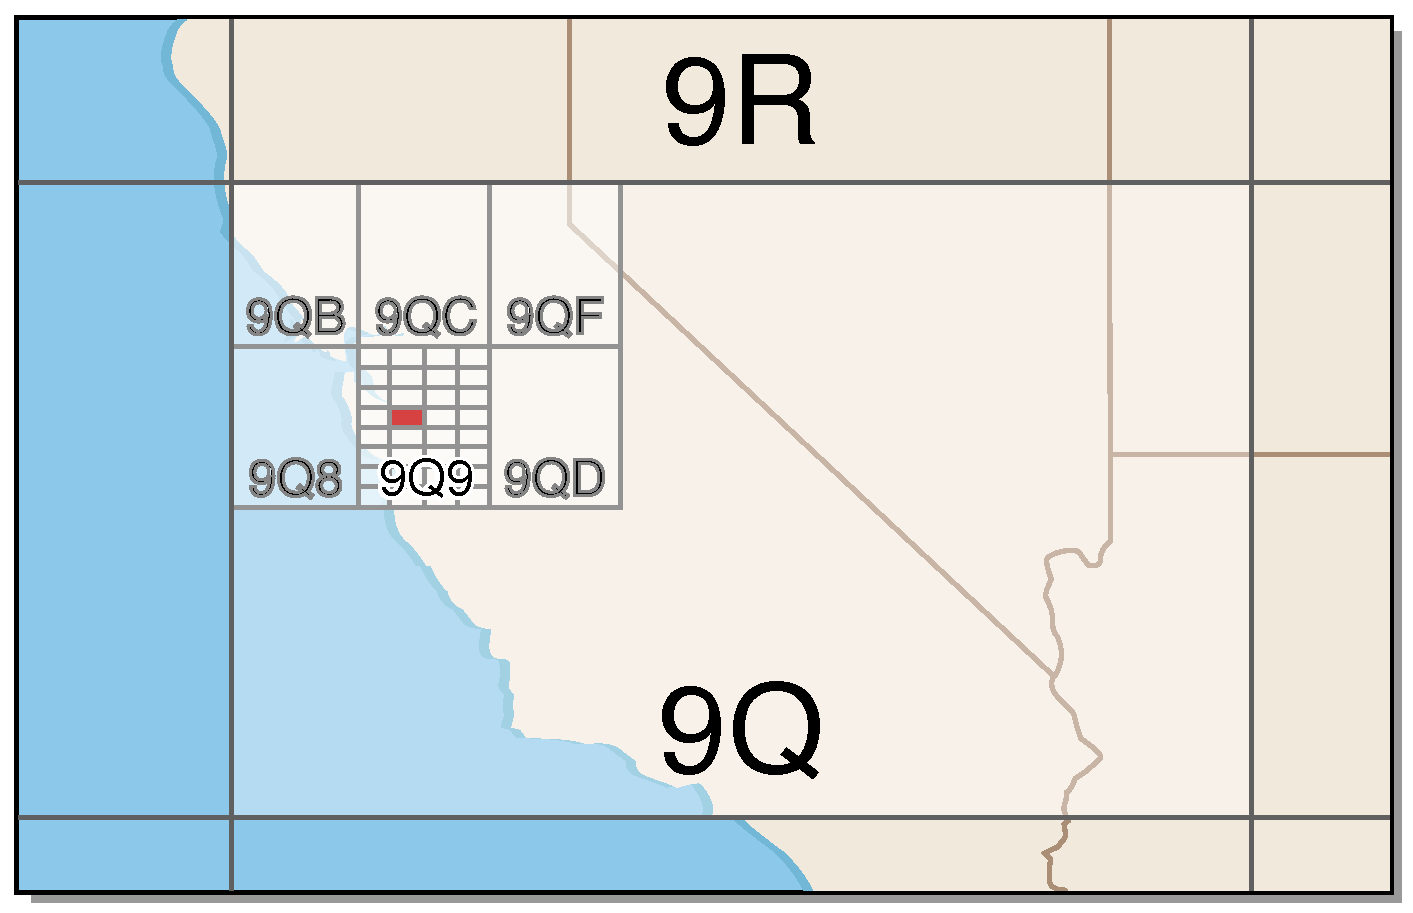
\includegraphics[width=3.5in]{figures/geohash.pdf}}
    \caption{A demonstration of the Geohash algorithm. Each additional character in a Geohash string describes a finer-grained region; Geohash \emph{DJ} contains substantial parts of Florida, Georgia, and Alabama, USA, while \emph{DJKJ} (highlighted in red) encompasses Tallahassee, the capital of Florida.}
    \label{fig:geohash}
\end{figure}

To achieve fine-grained control over our Geohash partitions, we operate at the bit level rather than Base 32 character level when routing streams. Each bit added to a Geohash string reduces its scope by half, with each character represented by five bits ($2^5 = 32$). In other words, a four-character Geohash string represents 20 spatial subdivisions. This property allows us to manage and allocate resources across a wide variety of observational densities.

Figure~\ref{fig:stream-partitioning} depicts a possible arrangement of the distributed sketch and the associated stream partitioning scheme corresponding to the same geographic region described above.
The distributed sketch is arranged in a tree-like structure.
Stream ingesters act as root nodes of this tree structure and they partition the geo-spatial stream among the \textsc{Synopsis} nodes using the Geohash based partitioning function.
Nodes closer to the root hold sketches corresponding to shorter Geohash strings.
In other words, they contain sketches for larger geographical regions.
For instance, nodes A and B in Figure~\ref{fig:stream-partitioning} are responsible for regions represented by Geohashes \emph{DJ} and and \emph{DN} respectively.
Node E, which is 3 edges deep from the stream ingester, is responsible for a smaller region, \emph{DJKJ}.

\textsc{Synopsis} is designed to ensure that the regions which are corresponding to larger portions of input streams, hence more frequent updates to the sketch, are moved to dedicated or less crowded nodes.
If a node decides to scale out a portion of the region it is currently responsible for, then the corresponding state (sketch and related meta data) is transferred over to the new computation and it starts to treat the stream packets corresponding to the scaled out region as pass-through traffic (Scaling out is explained in section~\ref{subsec:scaling-out}).
More specifically, it will not process the stream packet, instead updates its statistics based on the headers of the packet and forwards it to the child node . 
For instance, node A in Figure~\ref{fig:stream-partitioning} have scaled out two regions (\emph{DJK} and \emph{DJM}) to nodes C and D.
After these two scaling out operations, node A is responsible for all sub-regions in \emph{DJ} except for \emph{DJK} and \emph{DJM}.
Similarly the sketch for the region \emph{DJKJ} is moved out of node C into node E as a result of subsequent scale out operation.
It should be noted that the depth and span of the distributed sketch are dynamic and are constantly evolving according to the workload and operating conditions.

When the height of the tree grows, it becomes inefficient to have parent nodes passing through the traffic intended for the child nodes. 
Because it consumes extra bandwidth as well as increases the latency of the  corresponding sketch updates due to increased number of hops the packets have to travel through.
To circumvent this, we use short circuiting to direct traffic from stream ingesters straight to child nodes and avoid routing through parents.
This is depicted in Figure~\ref{fig:stream-partitioning} where stream ingester directly sends data to node E instead of sending it through nodes A and C.
We use our gossiping subsystem to update parents on the statistics related to child prefixes which are useful for scaling in decisions at later points of time as explained in section~\ref{subsec:scaling-out}.
Due to short circuiting, the data flow path starts to deviate from the tree like structure of the distributed sketch.

\begin{figure}
    \centerline{\includegraphics[width=3.5in]{figures/stream-partitioning.png}}
    \caption{An example of the stream partitioning based on Geohashes of the stream packets}
    \label{fig:stream-partitioning}
\end{figure}
 % This needs to be moved as we get the paper structure finalized

\subsection{Coping with High Data Rates: Scaling out}
\label{subsec:scaling-out}
There are two primary approaches to scaling a node that is experiencing high traffic: replication and load migration.   In replication-based scaling, during high data arrival rates, the original node spawns a new node that is responsible for identical spatial scopes as the original. Assimilation of the newly created node involves partitioning inbound streams directed to the original node. The upstream node is responsible for this partitioning, which may be performed in a skewed fashion with the new node receiving a larger portion of the inbound stream.  Alternatively, inbound streams to the original node may also be partitioned in a round-robin fashion between the original and the newly created node.

In targeted load migration, during heavy traffic the original node spawns a new node. However, in this case, particular geospatial scopes are evicted from the original node to the newly created node. The decision about the spatial scopes to be migrated is based on the data arrival rates and the rates at which particular portions of the sketch are being updated.

Replication-based scaling introduces a challenge during query evaluations in that the query must be forwarded to all nodes responsible for a particular scope and the results merged; depending on the nature of these queries (for e.g., correlation analysis and inferential queries) merging of results may be difficult to accomplish without extensive state synchronizations.
%TODO: lines about how downscaling can be difficult in replication settings

In \textsc{Synopsis}, we use targeted load migration for scaling out.
Our implementation closely follows the MAPE loop~\cite{maurer2011revealing} which is comprised of four phases: monitor (M), analyze (A), planning (P) and execution (E).
The monitoring task as shown in Figure~\ref{fig:process-monitor} periodically probes every \textsc{Synopsis} task to gather two performance metrics as part of monitoring phase.
\begin{enumerate}[leftmargin=*]
	\item Length of the backlog: This represents the number of unprocessed messages in the queue. If the \textsc{Synopsis} task cannot keep up with the incoming data rate, then the backlog will grow over time.
	\item Memory pressure: Each Neptune resource is a JVM process which is being allocated a fixed amount of memory. 
	Exceeding these memory limits create memory pressure which may cause extended garbage collection cycles and increased paging activity. 
	This will eventually lead to reduced performance in every  \textsc{Synopsis} task running in the Neptune resource.
	Monitoring task will continuously record the memory utilization by the entire JVM process as well as the memory utilization by individual \textsc{Synopsis} tasks.
\end{enumerate} 

The objective of scaling out is to maintain the stability of each node.
We define stability as the ability to keep up with incoming data rates while incurring a manageable memory pressure.

During the analysis phase, we use threshold based rules~\cite{lorido2012auto} to provide scale out recommendations to \textsc{Synopsis} nodes if necessary.
Currently we rely on a reactive scheme where we evaluate the threshold based rules based on the current observations.
Scaling out recommendations are provided if either of following rules are consistently satisfied for certain number of observations.
\begin{itemize}[leftmargin=*]  
\item Growing backlog - This is an indication that a portion of the load needs to be migrated to a different \textsc{Synopsis} node.
\item High overall memory utilization above a certain threshold (threshold is usually set below the memory limits allowing a capacity buffer for the process to avoid oscillation)
\end{itemize}

Upon receiving a scaling out recommendation from the monitoring task, a \textsc{Synopsis} node executes planning and execution phases.
During the planning phase, it will choose the portion(s) of the region within its current purview to be handed over to another node.
For this task, it relies on meta-data it maintains for each sub region (region corresponding to a longer Geohash string) and a numeric value provided along with the scale out recommendation which is a measure of how much load should be migrated.
This meta data includes the data rate and the timestamp of the last processed message for each sub region.
A \textsc{Synopsis} node updates these meta data with each message it processes.
Often a \textsc{Synopsis} node migrates several prefixes during a single scale out operation.

Only a single scale out operation takes place at a given time in a Neptune process.
This is controlled using a mutual exclusive lock (mutex) located in each Neptune process.
Further, every scaling operation is followed by a stabilization period where no scaling operation takes place and system does not enter the monitoring phase for the next MAPE cycle.
The objective of above constraints is to avoid oscillations in scaling activities.
For instance, if system aggressively scales out in the presence of a memory pressure without allowing a stabilization period, it is possible that the system ends up in a state where it is under provisioned. As a result of this, it will start aggressively scaling in and run again into an over provisioned state.

Figure~\ref{fig:scale-out-protocol} depicts the phases of the scale out protocol.
Once a \textsc{Synopsis} node decides on the sub regions, it initiates the scale out protocol by contacting the deployer.
In this message, it includes a list of preferred \textsc{Synopsis} nodes for the load migration as well as memory requirements and expected message rate for the load.
The preferred node set includes the \textsc{Synopsis} nodes that already holds its sub regions.
The objective is to minimize the number of \textsc{Synopsis} nodes responsible for holding sketches for a given geographical region, because it reduces the number of \textsc{Synopsis} nodes to contact during a query evaluation for that region.
Deployer has an approximate view of the entire system gathered through gossip messages which includes the memory pressure and cumulative backlog information of each node.
Based on this view and the information present in the request, deployer replies back with a set of target \textsc{Synopsis} nodes.
If it cannot find a suitable node out of the existing set, the deployer will launch a new \textsc{Synopsis} node and include its location in the new request.
Upon receiving the response from the deployer, \textsc{Synopsis} node contacts the target node and try to acquire the mutex.
Lock will be granted if no other scaling operations takes place in the Neptune process which holds the \textsc{Synopsis} node and it can accommodate the migrated load.
The second condition is checked again because the deployer may not have most upto-date metrics regarding the target \textsc{Synopsis} node due to the eventual consistent nature of its system view.
If the lock acquisition is failed, another node from the list of attempted.
Else the original \textsc{Synopsis} node will create a pass-through channel and direct traffic towards the target node.
In the same time, it will initiate a state transfer using a different channel in the background.
This will ensure that the state transfer doesn't affect the stream data flow and it happens asynchronously and the protocol ends without waiting for state transfer to complete.
Even if the state transfer is not complete, the target \textsc{Synopsis} node updates its memory utilization metric to account for the pending state transfer. 
Ending protocol within a short period of time is important because it can release mutual exclusive locks in both origin and target \textsc{Synopsis} nodes quickly and participate in other scaling activities soon after the stabilization period.
%
\begin{figure}
    \centerline{\includegraphics[scale=0.55]{figures/scale-out-protocol.png}}
    \caption{Scale out protocol}
    \label{fig:scale-out-protocol}
\end{figure}
%
\subsection{Downscaling}
During Scaling in, \textsc{Synopsis} nodes attempt to take back some of the sub-regions it scaled out previously to other \textsc{Synopsis} nodes.
This ensures better resource utilization in the system in addition to efficient query evaluations by having to contact less number of nodes.
Scaling in operations are also guarded by the same mutual exclusive lock used for scale out (only one scale out or scale in operation takes place at a given time) and followed by a stabilization period.

Monitoring and analysis phases are similar to scaling out scenario except for the obvious change to the threshold based rules.
Now both memory pressure and backlog length metrics should consistently record values below a predefined lower threshold.
When scaling in, we use a less aggressive scheme than scaling out; a single sub region is acquired during a single scale in operation.
Scaling in is more complex than scaling out because it deals with more than one \textsc{Synopsis} node in most cases.
Because at this point, it is possible that further scale out operations have taken place in the scaled out sub region after the initial scale out.
For instance, if node A in Figure~\ref{fig:stream-partitioning} decides to scale in the sub region \emph{DJK}, then it has to work with both nodes C and E.
Scale in protocol starts with a lock acquisition protocol similar to scale out protocol as illustrated in Figure~\ref{fig:scale-in-protocol}.
But it is required to lock the entire subtree where the sketch for the given sub region is distributed across.
As per our example, node A will have to acquire locks for nodes C and E.
Locks are acquired in a top-to-bottom fashion where parent locks itself and then attempts to lock the child.
If lock acquisition is failed in any part of the sub tree, then the scale in operation is aborted and the monitoring process will start the next iteration of the MAPE loop immediately.
If the sub tree is successfully locked, then data flow to the child nodes corresponding to this sub region is immediately terminated.
If there was a short circuit set up before, it will be removed and the data will start flow to the parent node.
The state acquisition phase begins next.
To ensure that \textsc{Synopsis} does not lose any messages, the initiator node sends a termination point control message to the child node.
Termination point is the sequence number of the last message sent to the child node either by the parent itself or by the short circuit channel.
It may be possible that the child has already processed this message and updated its sketch by the time it receives the termination point control message.
But in extreme cases, the termination point control message may get processed before the actual stream packet with the same sequence number.
This is because control plane and data plane use separate channels and also due to the possibility of data plane messages are being queued before processing.
Once the child node has processed every message up to the termination point, it sends out termination point messages to all relevant child nodes (In our example, node C sends a termination point control message to node E upon processing the stream packet corresponding to the termination point sent by node A).
After the entire sub tree has seen all messages up to the termination point, they acknowledge the initiator node and starts transferring their states asynchronously as similar to scale out protocol.
Once the parent node receives acknowledgments from the entire subtree, it starts propagating the protocol end messages to initiate lock releasing.
Locks are released from the bottom to top in the sub tree where parent releases its lock after noticing that every child participated in the scale in protocol has released its lock.

\begin{figure}
    \centerline{\includegraphics[scale=0.55]{figures/scale-in-protocol.png}}
    \caption{Scale in protocol}
    \label{fig:scale-in-protocol}
\end{figure}

\subsection{Query Evaluations}
\label{subsec:query-eval}
\textsc{Synopsis} incorporates support for user-defined queries that are evaluated over the distributed sketch.  Queries can be specified by the user in a SQL-like format or with JSON-based key-value descriptions similar to GraphQL~\cite{graphql}. Exact-match, range-based, and summarization queries are all supported over spatiotemporal bounds and individual feature values. The following example depicts how SQL-like queries can be formulated for evaluation over the sketch.

\begin{verbatim}
SELECT MEAN(precipitation), MAX(wind_speed)
WHERE temperature > 20 AND temperature < 30
AND humidity > .8 AND CORRELATION(
    cloud_cover, precipitation) < -0.25
\end{verbatim}

Depending on scaling operations and the spatial scope of the queries, evaluations are carried out on one or more sketchlets. Information on the placement of sketchlets in the system and their corresponding feature scopes is maintained at each sketchlet in a geohash prefix tree, with changes propagated through the network in an eventually-consistent manner as data is ingested and scaling maneuvers occur.

The entry point for these queries, called the \emph{conduit}, may be any of the sketchlets comprising the distributed sketch. During query evaluations, the first step is to identify the set of sketchlets that are relevant to the query. The conduit consults its prefix tree to locate sketchlets based on spatial, chronological, and feature constraints specified by the user. After this process is complete, the conduit forwards the queries on to the sketchlets for evaluation and supplies the client with a list of sketchlets that will respond to the query. As queries execute, results are streamed back to the client and merged by the client API. This strategy ensures that I/O and processing activities are interleaved on the client side.

Our distributed prefix tree enables query evaluations during both scaling in and out. For instance, when a conduit attempts to forward a query to a child sketchlet that is undergoing a scale-in operation, the request will be redirected to the its parent sketchlet. This process can continue recursively up through the network, ensuring queries will reach their destination.

\subsubsection{Query Types}
Queries supported by \textsc{Synopsis} fall into six categories:

\begin{description}[leftmargin=*]
    \item[Relational Queries] describe the feature space in the context of the hierarchical trees within our SIFT data structure and may target ranges of values under certain conditions. For example, ``What is the relationship between temperature and humidity during July in Alaska, USA, when precipitation was greater than 1 centimeter?'' These queries return a subset of the overall sketch that includes other matching feature values as well.
    % Subsketches may be manipulated and inspected on the client side, and then reused in subsequent queries to request more detail or broaden the query scope. Relational queries can optionally return statistical metadata stored in the leaf nodes of the tree; this is also supported by our statistical query functionality.

    \item[Statistical Queries] allow users to explore statistical properties of the observational space by retrieving portions of the metadata stored in the leaf nodes of the sketch. For example, users can retrieve and contrast correlations between any two features at different geographic locations at the same time. Alternatively, queries may contrast correlations between different features at different time ranges at the same geographic location. These queries also support retrieval of the mean, standard deviation, and feature outliers based on Chebyshev's inequality \cite{knuth1968art}.

    \item[Density Queries] support analysis of the distribution of values associated with a feature over a particular spatiotemporal scope. These include kernel density estimations, estimating the probability of observing a particular value for an observation, and determining the deciles and quartiles for the observed feature.% Kernel density estimations can request the function itself, an integral over a range of values, or the probability of a single value.

    \item[Set Queries] target identification of whether a particular combination of feature values was observed, estimating the cardinality of the dataset, and identifying the frequencies of the observations. Each type of set query requires a particular data structure, with instances created across configurable time bounds (for instance, every day). Set membership is determined using space-efficient bloom~filters~\cite{bloom1970space}, while cardinality (number of distinct elements) queries are supported by the HyperLogLog~\cite{flajolet2007hyperloglog} algorithm.

%To determine set membership, we use Bloom filters may produce false positives, but never false negatives. Besides returning a \texttt{true} or \texttt{false} result to the user, membership queries also include the probability of the answer being a false positive.  Set HyperLogLog is able to estimate cardinality with high accuracy and low memory consumption. Finally, observation frequencies are provided by the count-min data structure \cite{cormode2005improved}. Count-min is structurally similar to a bloom filter, but can be used to estimate the frequency of values within a particular error band. Frequency queries are accompanied by their associated confidence intervals and relative error.

\item[Inferential Queries]
    Inferential queries enable spatiotemporal forecasts to be produced for a particular feature (or set of features). Discrete inferential queries leverage existing information in the distributed sketch to make predictions; aggregate metadata stored in the leaves of the tree can produce two-dimensional regression models that forecast new outcomes across each feature type when an independent variable of interest changes.

%In their continuous form, inferential queries are backed by machine learning models that are \emph{installed} for a particular time window and can be trained using either the sketch or new, full-resolution values as they arrive. Continuous inferential queries can stream predictions back to the client on a regular interval, or a subsequent query can reference a particular model and parameterize it to make a single prediction. Our current implementation of \textsc{Synopsis} supports multiple linear regression, but our machine learning interface allows new models to be plugged into the system at run time.

\item[Synthetic Data Queries] allow users to request the system to generate representative datasets based on the distributions stored in the sketch. Synthetic data is generated in an online fashion by sampling from the underlying distributions and then streamed to client applications for analytics. The size of the dataset may also be specified; for instance, 10\% of the volume of the original data points.
\end{description}

Table~\ref{tbl:query-times} outlines local tree traversal times for query evaluations. These queries were separated into two groups: conventional lookups and tree retrievals. Conventional lookups include density queries, set queries, and statistical queries, while tree retrievals request targeted portions of the overall feature space as a tree.  Note that while conventional lookups do not return a tree structure to the client, they still require a tree traversal to resolve. In general, tree retrievals consume more processing time due to their serialization and I/O costs; however, it is worth noting that varying the geographical scope across sketchlet sizes from 5km to 800km did not result in a proportionate increase in processing time. Overall, the sketch is able to satisfy our goal of low-latency query evaluations for each query type.

\begin{table}[b]
    \renewcommand{\arraystretch}{1.4}
    \caption{Local sketchlet evaluation times for each query type (averaged over 1000 iterations). \vspace{-1em}}
    \label{tbl:query-times}
    \begin{center}
        \begin{tabular}{|l|c|c|}
            \hline
            \textbf{Query Type}      & \textbf{Eval. (ms)} & \textbf{Std. Dev.} \\
            \hline
            Density                  & 0.007                    & 0.005 \\
            \hline
            Set Cardinality          & 0.154                    & 0.088 \\
            \hline
            Set Frequency            & 0.036                    & 0.019 \\
            \hline
            Set Membership           & 0.015                    & 0.009 \\
            \hline
            Statistical               & 0.002                    & 0.001 \\
            \hline
            \hline
            Tree Only (5 km)        & 46.357                   & 1.287 \\
            \hline
            Tree + Meta (5 km)      & 40.510                   & 6.937 \\
            \hline
            Tree + Meta (25 km)     & 47.619                   & 6.355 \\
            \hline
            Tree + Meta (800 km)    & 53.620                   & 6.818 \\
            \hline
        \end{tabular}
    \end{center}
\end{table}


\subsection{Coping with Failures in \textsc{Synopsis}}
\textsc{Synopsis} relies on passive replication to recover from sketchlet failures.
Other techniques such as active replication increase the resource consumption significantly and it is infeasible to use upstream backups because the state of a Sketchlet depends on the entire set of stream packets it has processed previously \cite{castro2013integrating}.

Support for fault tolerance is implemented by augmenting the distributed sketch) with a set of secondary sketchlets.
Each sketchlet is assigned with a set of $n$ secondary sketchlets each running on different machines, so that Synopsis can withstand up to $n$ concurrent machine failures.
In our implementation, we used two secondary sketchlets assigned to each sketchlet.
The primary sketchlet periodically sends the changes to its in-memory state to the secondary nodes creating an stream of edits to the sketchlet between the primary and secondary sketchlets.
This incremental check-pointing scheme consumes a less bandwidth compared to a periodic check-pointing scheme that replicates the entire state every time \cite{castro2013integrating}.
The secondary sketchlets, which acts as the sink to the edit stream serializes the messages received via the edit stream to persistent storage.
By default, \textsc{Synopsis} uses the disk of the machine which hosts the secondary sketchlet for persistent storage, but necessary API level provisions are included to support highly available storage implementations such as HDFS~\cite{borthakur2008hdfs}.
To reduce the overhead caused by secondary sketchlets, they do not load this serialized state into its memory unless there is a failure to the primary and consequently it gets appointed as the primary sketchlet using the leader election protocol implemented using Zookeeper~\cite{hunt2010zookeeper}.

Incremental checkpoints are performed based on a special control message emitted by the stream ingesters.
These messages help to orchestrate a system-wide incremental checkpoint.
\textsc{Synopsis} uses upstream backups at stream ingesters to keep a copy of the messages that entered the system since the last successful checkpoint.
In case of a failure, all messages since the last checkpoint will be replayed.

A sketchlet is implemented as an idempotent data structure using message sequence numbers, hence it will process a replayed message only if the message is not processed before.
Users can apply their own policy for defining the interval between the incremental checkpoints based on time or the number of emitted messages.
Frequent checkpoints can incur high overhead whereas longer periods between successive checkpoints may consume more resources for upstream backups as well as for replaying messages in case of a failure.

Membership management is implemented using Zookeeper, which is leveraged to detect failed nodes.
Upon receiving node failure notifications, a secondary sketchlet is assumed the role of the primary.
The secondary will start processing messages immediately and start populating its state from the persistent storage in the background.
Given this mode of operation, there may be a small window of time during which the correctness of queries are impacted.
This is rectified once the stored state is loaded to memory and replay of the upstream backup is completed.
The sketch's ability to correctly process out of order messages and support for merging with other sketches is useful during this failure recovery process.

As per our fault tolerance model, the \textit{total time to recover from the failure} ($T_{total}$) can be modeled by the following equation.
\begin{align*}
    T_{total} &= T_{d} + \max{(T_{l}, T_{r})}      
\end{align*}
where $T_{d}$ = \textit{time to detect a failure}, $T_{l}$ = \textit{time to load persisted state} and $T_{r}$ = \textit{replay time for messages at the upstream node}.

Time to detect failure mainly depends on the session timeout value used by the Zookeeper to detect lost nodes and the delay in propagating the notification about the lost cluster-node to other members. With a $5s$ session timeout in an active cluster, we observed a mean notification propagation delay of $5.500s$ (std. deviation = $0.911s$, $95^{th}$ Percentile = $6.000s$). Configuring a lower session timeout will increase the chance of false negatives if cluster-nodes become non responsive for a while due to increased load or system activities such as garbage collection. Using a higher session timeout will increase the time to detect failures. Time required to load the persisted storage depends on the size of the serialized sketchlet. We benchmarked the time it takes to repopulate the state in all sketchlets after ingesting NOAA data for year 2014. The mean state re-population time was recorded as $16.602s$ with a std. deviation of $23.215s$ and a $95^{th}$ percentile of $70.877s$. Replay time mainly depends on the check-pointing interval as well as the message ingestion rate. With a check-pointing interval of 10000 messages, we experienced a mean value of $0.447s$ (std. deviation = $0.036s$, $95^{th}$ Percentile = $0.484s$) to replay the buffered messages from stream ingesters.  														





\section{Performance Evaluation}
Here we report system benchmarks profiling several aspects of \textsc{Synopsis}. This includes: memory consumption of the sketch, data ingestion performance of the sketch, ability to handle variable loads, organization of the sketchlets within the sketch and its query evaluation performance.
\label{sec:performance}
\subsection{Dataset and Experimental Setup}
Our subject dataset was sourced from the NOAA North American Mesoscale (NAM) Forecast System \cite{noaa_nam}.  The NAM collects atmospheric data several times per day and includes features of interest such as surface temperature, visibility, relative humidity, snow, and precipitation. Each observation in the dataset also incorporates a relevant geographical location and time of creation. This information is used during the data ingest process to partition streams across available computing resources and preserve temporal ordering of events. The size of the entire source dataset was 25 TB.

Performance evaluations reported here were carried out on a cluster of 40 HP DL160 servers (Xeon E5620, 12 GB RAM). The test cluster was configured to run Fedora 24, and \textsc{Synopsis} was executed under the OpenJDK Java runtime 1.8.0\_72.
%
%
\begin{figure}[t!]
    \centerline{\includegraphics[width=\linewidth]{figures/ing-and-mem-usage.pdf}}
    \caption{Memory usage of the distributed sketch over time against the amount of ingested data. The rate of growth decreases over time due to the compact nature of sketchlet data structure.}
    \label{fig:dist-sketch-mem-usage}
\end{figure}
%
%
\subsection{Distributed Sketch Memory Evaluation}
\begin{table*}[h]
    \renewcommand{\arraystretch}{1.3}
    \caption{Profiling the update performance of sketchlet and sketch at high data ingest rates}
    \label{tab:throughput}
    \begin{center}
        \begin{tabularx}{0.9\textwidth}{|X|c|c|c|c|c|c|c|}
            \hline
            \multirow{2}{*}{Ingester Count} & \multicolumn{2}{c|}{\cellcolor[gray]{0.7}Sketchlet Throughput (msgs/s)} &\multicolumn{2}{c|}{\cellcolor[gray]{0.7}Sketch Throughput (msgs/s)} & \multicolumn{3}{c|}{\cellcolor[gray]{0.7}Sketchlet Update Latency (ns)} \\
            \cline{2-5}
             & \cellcolor[gray]{0.9}Mean & \cellcolor[gray]{0.9}Std. Dev.  &  \cellcolor[gray]{0.9}Mean & \cellcolor[gray]{0.9}Std. Dev.
             &  \cellcolor[gray]{0.9}Mean & \cellcolor[gray]{0.9}$95^{th}$ Perc. & \cellcolor[gray]{0.9}Std. Dev. \\
            \hline
            1 & 15124.562 & 575.728 & 44082.476 & 5984.503 & 64752.413 & 67175.250 & 5503.007 \\
            \hline
            2 & 14067.452 & 491.783 & 44060.889 & 6206.208 & 64971.289 & 71170.200 & 4012.358 \\
            \hline
            4 & 11319.321 & 1003.462 & 41645.317 & 13553.462 & 74025.649 & 78364.100 & 3124.570 \\
            \hline
            8 & 5223.280 & 717.254 & 38369.745 & 14008.308 & 81034.038 & 85842.400 & 2501.929 \\
            \hline
        \end{tabularx}
    \end{center}
\end{table*}
%
We monitored the growth in memory consumption of the entire distributed sketch over time with continuous data ingestion as shown in Figure~\ref{fig:dist-sketch-mem-usage}. As more data was streamed into the system, the growth rate of the distributed sketch decreased as the sketchlets expanded to include vertices for their particular feature space.  At the end of our monitoring period, the total amount of ingested data was over three orders of magnitudes higher ($\sim 1285$) than the in-memory sketch size, resulting in notable space savings.
\subsection{Sketch Ingestion Rate}
In this experiment, we assessed the ability of the sketch to keep pace with the high rates of incoming observational streams.
We partitioned our dataset based on timestamps of observations such that each partition comprised observations for a contiguous time period.
Within a partition, data collected in a single observation cycle for all geographical locations were stored as successive records.
Records within a single observation cycle were stored in the same order based on their locations across all observational cycles in all partitions.
Each partition was assigned a single ingester that sequentially parsed and streamed these records to the distributed sketch.
This organization of observations ensured that multiple stream ingesters target a small subset of the sketchlets to profile the \textit{worst case} performance under high stress.
This setup forces the corresponding SIFT trees to fan-out on different planes (time and features) simultaneously representing a strenuous workload on the sketch where different sections within the sketch will be stress tested over time.
A real world scenario is simulated with a single partition.

Table~\ref{tab:throughput} summarizes the results of this benchmark.
As we increase the number of ingesters with a single sketchlet, the throughput decreases due to the simultaneous fan-out operations taking place within the SIFT trees. This claim is further supported by the increase in the latency for updating the sketchlet as shown in the table.

For the sketch, we started with a single sketchlet and allowed the system to dynamically scale out and measured its throughput once it becomes stable --- when there are no frequent scaling activities.
System reached the stable state with 14-16 sketchlets in different setups.
We observed a higher throughput compared to the performance of a single sketchlet due to parallel processing of the observational stream but it did not increase linearly with the number of sketchlets.
When there is a single ingester, the throughput was constrained by the bandwidth of the machine where the ingester was running --- we were using around 86\% of the available bandwidth.
With multiple ingesters, due to the way the stream is (intentionally) constructed, the load is not evenly partitioned across the cluster at a given time --- only a subset of sketchlets were processing the stream.
%
\subsection{Dynamic Scaling: Responding to Variable Load}
\begin{figure}[t!]
    \centerline{\includegraphics[width=3.5in]{figures/dyn-scaling.pdf}}
    \caption{Variation in the number of sketchlets as the data ingestion rate changes.}
    \label{fig:dyn-scaling}
\end{figure}
We evaluated how \textsc{Synopsis} dynamically scales when the data ingestion rate is varied.
The data ingestion rate was varied over time such that the peak data ingestion rate is higher than the highest possible cumulative throughput to create a backlog at sketchlets.
We augmented the sketch update code with additional operations to match the relatively low ingestion rates used for better control.
We used the number of sketchlets within the system to quantify the scaling activities.
If the system scales out, more sketchlets will be created as a result of targeted load migration.
We started with a single sketchlet and allowed the system to dynamically scale.
As can be observed in Figure~\ref{fig:dyn-scaling}, the number of sketchlets varies with the ingestion rate.
Since we allow aggressive scale-out, rapid scaling out is observed during high data ingestion rates whereas scaling in takes place gradually with one subregion (one sketchlet) at a time.

\subsection{Analyzing a Snapshot of the Distributed Sketch}
% scale out graph
\begin{figure*}[h!]
    \centerline{\includegraphics[width=\linewidth]{figures/scaleout_graph_analysis.pdf}}
    \caption{Analysis of a snapshot of the distributed sketch during data ingestion demonstrating the size and distribution of the information corresponding to different prefixes against the observed record count. If the information is dispersed over multiple sketchlets, it is likely to be a prefix with higher number of records and/or a wide range of observed values.}
    \label{fig:scaleout-graph-analysis}
\end{figure*}
%
Figure~\ref{fig:scaleout-graph-analysis} visualizes a snapshot of the distributed sketch which demonstrates the organization of sketchlets in runtime as described in \S\ref{sec:methodology}. 
This represents the state of the system after consuming the complete 2014 NOAA dataset and the sketch contained 48 sketchlets. 
It shows the distribution and size of the information maintained across sketchlets for each geohash prefix of length 3 against the number of records processed for that particular prefix.
The memory requirement for a particular geohash prefix depends on the number of records as well as the range of the observed values for different features.
The space requirement is measured by the number of leaf nodes in the corresponding sketchlets.
For the majority of the prefixes, the space requirement increases with the number of records processed.
If the data for a particular prefix is distributed across multiple sketchlets, then it is more likely to be a prefix with a high number of records as shown in the first subplot.
In such cases, some of these sketchlets are created in multiple iterations of scaling out operations from their original sketchlets which results in a higher distance from the root of the prefix tree. This is depicted in the second sub figure of Figure~\ref{fig:scaleout-graph-analysis}.
A few prefixes with high number of records can be observed with a low memory consumption and are distributed across multiple sketchlets.
Their observations spans across a smaller range, hence requires less memory but they were chosen for scaling out operations due to their high message rates. 


\subsection{Query Evaluation Performance}
\begin{figure*}[t!]
    \centerline{\includegraphics[width=\linewidth]{figures/query_benchmark_both.pdf}}
    \caption{Distributed query evaluation performance --- cumulative throughput and latency in a 40 node \textsc{Synopsis} cluster.}
    \label{fig:dist-query}
\end{figure*}
To evaluate distributed query performance, we executed several representative workloads across a variety of sketchlet sizes. These queries were separated into two groups: conventional lookups and tree retrievals.  Figure~\ref{fig:dist-query} depicts the end-to-end efficiency of the query evaluations over the distributed sketch.
Cumulative query throughput and latencies were measured with varying numbers of \emph{concurrent query funnels}.
A query funnel continuously generates and dispatches random queries at its maximum possible rate to stress test the system and saturate its capacity; for example, a query could request summary statistics or feature relationships when the temperature is between 20 to 30 degrees, humidity is above 80\%, and the wind is blowing at 16 km/h.
These randomized queries fluctuated in both the ranges of values and spatial scope, resulting in high variability in the number of sketchlets required to resolve the query as well as the depth and breadth of the required tree traversals.





\section{Applications}
\label{sec:applications}
To demonstrate the effectiveness of \textsc{Synopsis} as a surrogate for the data, we profile its use in two settings normally under the purview of on-disk data: visualization and analytical computations.
\subsection{Visualization}
To demonstrate the potential applications of Synopsis, we created two representative visualizations. Our first visualization generated a climate chart by issuing statistical queries to retrieve high, low, and mean temperature values as well as precipitation information for a given spatial region. Climate charts are often used to provide a quick overview of the weather for a location; Figure~\ref{fig:climate} summarizes the temperature and precipitation in Snowmass Village, Colorado during 2014. While a standard approach for producing these visualizations over voluminous atmospheric data would likely involve several MapReduce computations, our sketchlets make all the necessary information readily available through queries, avoiding distributed computations altogether.

\begin{figure}[h]
    \centerline{\includegraphics[width=\linewidth]{figures/climate-snowmass.pdf}}
    \caption{Climate chart visualization}
    \label{fig:climate}
\end{figure}

Our second visualization ...

\begin{figure}[h]
    \centerline{\includegraphics[width=2.85in]{figures/globe.pdf}}
    \caption{Global contour visualization}
    \label{fig:global-contour}
\end{figure}

\subsection{Use with Analytic Engines}
\textsc{Synopsis} can be used to generate synthetic data that requires less space while providing an effective representation of the actual data.
Such synthetic datasets can be used efficiently with analytic engines such as Spark and Tensorflow.

We used Apache Spark to train a regression model based on Random Forests ensemble method to predict temperature using surface visibility, humidity and precipitation.
Different models were generated using the actual data and synthetic data sets representing 10\% and 20\% of the actual data.
The accuracy of these models were measured using the a test dataset extracted from actual observations.
The data was staged on HDFS and loaded into Spark to train the ensemble models.
%
\begin{table*}
    \renewcommand{\arraystretch}{1.3}
    \caption{Comparing Random Forest based regression models generated by Spark MLlib using synthetic vs. real data}
    \label{tab:spark-rf}
    \begin{center}
        \begin{tabularx}{0.98\textwidth}{|X|X|X|c|c|c|c|c|c|}
            \hline
            \multirow{2}{*}{Dataset} & \multirow{2}{*}{Size (GB)} & \multirow{2}{*}{RDD Partitions Count} & \multicolumn{2}{c|}{\cellcolor[gray]{0.7}Data Loading Time (s)} &\multicolumn{2}{c|}{\cellcolor[gray]{0.7}Model Training Time (s)} & \multicolumn{2}{c|}{\cellcolor[gray]{0.7}Accuracy (RMSE)}\\
            \cline{4-9}
             & & & \cellcolor[gray]{0.9}Mean & \cellcolor[gray]{0.9}Std. Dev.  &  \cellcolor[gray]{0.9}Mean & \cellcolor[gray]{0.9}Std. Dev. &  \cellcolor[gray]{0.9}Mean & \cellcolor[gray]{0.9}Std. Dev. \\
            \hline
            Original Data & 25.350 & 208 & 4.611 & 0.133 & 520.657 & 7.690 & 6.025 & 0.051 \\
            \hline
            Synthetic Data - 10\% & 2.549 & 21 & 3.424 & 0.288 & 246.212 & 15.046 & 5.980 & 0.024 \\
            \hline
            Synthetic Data - 20\% & 4.336 & 41 & 3.997 & 0.392 & 278.682 & 17.475 & 6.018 & 0.064 \\
            \hline
		\end{tabularx}
	\end{center}
\end{table*}
%
We evaluated the efficacy of our approach based on the on-disk and in-memory storage requirements, data loading time, training time and the accuracy of the model.

Our observations are summarized in table~\ref{tab:spark-rf}.
The accuracy of the models generated based on synthetic data is comparable to the accuracy of the models generated using actual data.
But they require less space and reduces the training time significantly.
For instance, 10\% synthetic dataset produces a model with similar accuracy incurring 53\% less training time while reducing the space requirement by 90\%. 



\subsection{Use with Analytic Engines}
\textsc{Synopsis} can be used to generate synthetic data that requires less space while providing an effective representation of the actual data.
Such synthetic datasets can be used efficiently with analytic engines such as Spark and Tensorflow.

We used Apache Spark to train a regression model based on Random Forests ensemble method to predict temperature using surface visibility, humidity and precipitation.
Different models were generated using the actual data and synthetic data sets representing 10\% and 20\% of the actual data.
The accuracy of these models were measured using the a test dataset extracted from actual observations.
The data was staged on HDFS and loaded into Spark to train the ensemble models.
%
\begin{table*}
    \renewcommand{\arraystretch}{1.3}
    \caption{Comparing Random Forest based regression models generated by Spark MLlib using synthetic vs. real data}
    \label{tab:spark-rf}
    \begin{center}
        \begin{tabularx}{0.98\textwidth}{|X|X|X|c|c|c|c|c|c|}
            \hline
            \multirow{2}{*}{Dataset} & \multirow{2}{*}{Size (GB)} & \multirow{2}{*}{RDD Partitions Count} & \multicolumn{2}{c|}{\cellcolor[gray]{0.7}Data Loading Time (s)} &\multicolumn{2}{c|}{\cellcolor[gray]{0.7}Model Training Time (s)} & \multicolumn{2}{c|}{\cellcolor[gray]{0.7}Accuracy (RMSE)}\\
            \cline{4-9}
             & & & \cellcolor[gray]{0.9}Mean & \cellcolor[gray]{0.9}Std. Dev.  &  \cellcolor[gray]{0.9}Mean & \cellcolor[gray]{0.9}Std. Dev. &  \cellcolor[gray]{0.9}Mean & \cellcolor[gray]{0.9}Std. Dev. \\
            \hline
            Original Data & 25.350 & 208 & 4.611 & 0.133 & 520.657 & 7.690 & 6.025 & 0.051 \\
            \hline
            Synthetic Data - 10\% & 2.549 & 21 & 3.424 & 0.288 & 246.212 & 15.046 & 5.980 & 0.024 \\
            \hline
            Synthetic Data - 20\% & 4.336 & 41 & 3.997 & 0.392 & 278.682 & 17.475 & 6.018 & 0.064 \\
            \hline
		\end{tabularx}
	\end{center}
\end{table*}
%
We evaluated the efficacy of our approach based on the on-disk and in-memory storage requirements, data loading time, training time and the accuracy of the model.

Our observations are summarized in table~\ref{tab:spark-rf}.
The accuracy of the models generated based on synthetic data is comparable to the accuracy of the models generated using actual data.
But they require less space and reduces the training time significantly.
For instance, 10\% synthetic dataset produces a model with similar accuracy incurring 53\% less training time while reducing the space requirement by 90\%. 


\section{Related Work}
\label{sec:related}

Galileo \cite{} is a distributed hash table that supports the storage and retrieval of multidimensional data. Given the overlap in problem domain, Galileo is faced with several of the same challenges as \textsc{Synopsis}. However, the avenues for overcoming these issues diverge significantly due to differences in storage philosophy: \textsc{Synopsis} maintains its dataset completely in main memory, avoiding the orders-of-magnitude disparity in I/O throughput associated with secondary storage systems. This makes \textsc{Synopsis} highly agile, allowing on-demand scaling to rapidly respond to changes in incoming load. Additionally, this constraint influenced the trade-off space involved when designing our algorithms, making careful and efficient memory management a priority while striving for high accuracy.

Dynamic scaling and elasticity in stream processing systems are studied before~\cite{heinze2014auto, gulisano2012streamcloud, castro2013integrating, loesing2012stormy, heinze2013elastic, schneider2009elastic}.
Heinze et al.~\cite{heinze2014auto} have explored using different dynamic scaling schemes including threshold based rules and reinforcement learning using the FUGU~\cite{heinze2013elastic} stream processing engine.
Based on these schemes, the operators are continuously migrated between hosts in a FUGU cluster in order to optimize the resource utilization and to maintain a low latency.
Their approach is quite different from ours, because in \textsc{Synopsis} we perform a targeted load migration where the workload of a computation is dynamically adjusted instead of entirely moving it to a host with a higher or lower capacity than the current host.
Further we do not interrupt the data flow through \textsc{Synopsis} when dynamic scaling activities are in progress whereas in FUGU predecessor operator is temporarily paused until the operator migration is complete. 
StreamCloud~\cite{gulisano2012streamcloud} relies on a global threshold based scheme to implement elasticity where a query is partioned into sub-queries which run on separate clusters.
StreamCloud relies on a centralized component, Elastic Manager, to initiate the elastic reconfiguration protocol whereas in Synopsis each node independently initiates the dynamic scaling protocol.
This difference is mainly due to different optimization objectives of the two systems; StreamCloud tries to optimize the average CPU usage per cluster while Synopsis attempts to maintain stability at each node.
State recreation protocol of StreamCloud is conceptually similar to the state transfer protocol in Synopsis, except in StreamCloud the tuples are buffered at the new location until the state transfer is complete.
But in Synopsis, the new node starts building the state (sketch) which is later merged with the asynchronously transferred state from the previous node.
Gedik et al.~\cite{schneider2009elastic} also uses a threshold based local scheme similar to \textsc{Synopsis}; additionally they keep track of the past performance achieved at different operating conditions in order to avoid oscillations in scaling activities.
The use of consistent hashing at the splitters (similar to stream partitioners of \textsc{Synopsis}) achieves both load balancing and monotonicity (elastic scaling does not move states between nodes that are present before and after the scaling activity).
Similarly, Geohash based partitioner together with control algorithm in Synopsis balance the workload by alleviating hotspots and nodes with lower resource utilization.
Also our state migration scheme doesn't require migrating states between nodes who do not participate in the scaling activity unlike with a reconfiguration of a regular hash based partitioning.
Unlike in Synopsis, in their implementation, the stream data flow is paused until state migration is complete using vertical and horizontal barriers.
Also Synopsis' scaling schemes are placement-aware; which prefers certain nodes when performing scaling activities with the objective of reducing the span of the distributed sketch.


\section{Conclusions and Future Work}
\label{sec:conclusions}
In this paper, we presented a framework for constructing a distributed sketch over spatiotemporal observational streams. \textsc{Synopsis} maintains compact representation of the observational space, supports dynamic upscaling and downscaling to preserve responsiveness and avoid overprovisioning, and supports a rich set of queries to explore the observational space. Our methodology for achieving this is broadly applicable to other stream processing systems.  Our empirical benchmarks, with real-world observational data, demonstrate the suitability of our approach.We now make a set of assertions pertaining to the research questions that we explored in this study.
\begin{description}[leftmargin=*]
\item[RQ-1:] Extracting metadata from observational data streams as they come in. We then check to see if the sketch needs to be updated. Each vertex represents a range of values; 
We achieve compactness because the number of vertices in the graph is influenced by the number of ranges and how they are organized both of which are dynamically managed in \textsc{Synopsis} using density-driven quantization.  We also maintain summary statistics within these vertices to track the distribution/dispersion of feature values and the frequency with values fall within that range. Maintaining such summary statistics in an online fashion precludes the need to maintain fine-grained information that is memory intensive.

\item[RQ-2:] Data arrivals in observational settings are not uniform and the underlying infrastructure must be responsive to it.  There will be variability in the rates and volumes of data arrivals from different geolocations due to differences and flux in the number of sensing sources. \textsc{Synopsis} scaling mechanism avoid overprovisioning via targeted scaling of portions of \textsc{Synopsis}. 
Targeted scaling allows us to alleviate situations where sketch updates cannot keep pace with data arrival rates.  Memory pressure is also taken into account during upscaling, downscaling, and creation of spares. Since \textsc{Synopsis} is memory-resident (to avoid disk I/O costs) tracking strains induced either by nodes comprising the \textsc{Synopsis} distributed sketch or the collocated processes is critical.

Given the rates of data arrivals, reactive schemes for scaling would result in updates and query evaluations over portions of the feature space to be slow. Our proactive scaling scheme triggers dynamic upscaling and downscaling based on the expected data arrival rates and the accompanying memory footprints. Our distributed locking scheme avoid deadlocks and liveness issues during scaling operations.

\item[RQ-3:] \textsc{Synopsis} is spatially explicit, with nodes comprising distributed sketch responsible for managing particular geospatial scopes. Scaling decisions are localized to particular nodes and involve load shedding during upscaling and fusion during downscaling. Each \textsc{Synopsis} node also maintains a prefix tree that maintains compact information about the nodes managing geospatial scopes. At each node, the metadata graph maintains information about different chronological time ranges; the system maintains fine-grained information about recent data and coarser grained information about older, historical data. This structure supports incremental scaling, allows nodes to effectively assimilate observations at high rates, and redirect queries to nodes where they should be evaluated. Our graph based organization of the extracted metadata allows us to support a rich set of queries without compromising on timeliness; the accuracy of these evaluations is influenced by the granularity of the representations.  

\item[RQ-4:] Since we support targeted upscaling and downscaling based on the data arrival rates and memory pressure, the assimilations and query evaluations can keep pace with the observations. During query evaluations,  only those \textsc{Synopsis} nodes that hold portions of the observational space implicitly or explicitly targeted by the query are involved in the query evaluations, and that to independently and without synchronizing with each other: this allows us to support high throughput query evaluations.

Our future work will target support for \textsc{Synopsis} to be used as input for long-running computations that are expressed as MapReduce jobs. Such jobs that would execute periodically and on potentially varying number of machines could target the entire observational space or only the most recent ones.
\end{description}

\vspace{1em}\\
\section*{Acknowledgments}
This research has been supported by funding (HSHQDC-13-C-B0018 and D15PC00279) from the US Department of Homeland Security, the US National Science Foundation's Computer Systems Research Program (CNS-1253908), and the Environmental Defense Fund (0164-000000-10410-100). \\


% ensure same length columns on last page (might need two sub-sequent latex runs)
% \balance

\bibliographystyle{IEEEtran}
\bibliography{references}
\vspace*{-3.7\baselineskip}
\begin{IEEEbiography}[{\includegraphics[width=1in,height=1.2in, clip,keepaspectratio]{./bio/thilina.jpg}}]{Thilina Buddhika} is a Ph.D. candidate in the Computer Science department at Colorado State University.  His research interests are in the area of real time, high throughput stream processing specifically targeted to environments such as Internet of Things (IoT) and health care applications. Email: thilinab@cs.colostate.edu
\end{IEEEbiography}
\vspace{-1.60cm}
\begin{IEEEbiography}[{\includegraphics[width=1in,height=1.2in,clip,keepaspectratio]{./bio/matthew.jpg}}]{Matthew Malensek} is a Ph.D. student in the Department of Computer Science at Colorado State University. His research involves the design and implementation of large-scale distributed systems, data-intensive computing, and cloud computing. Email: malensek@cs.colostate.edu
\end{IEEEbiography}
%
\vspace{-1.60cm}
\begin{IEEEbiography}[{\includegraphics[width=1in,height=1.2in,clip,keepaspectratio]{./bio/sangmi.jpg}}]{Sangmi Lee Pallickara} is an Assistant Professor in the Department of Computer Science at Colorado State University. She received her Masters and Ph.D. degrees in Computer Science from Syracuse University and Florida State University, respectively. Her research interests are in the area of large-scale scientific data management. She is a recipient of the NSF CAREER award. Email: sangmi@cs.colostate.edu
\end{IEEEbiography}
%
\vspace{-1.56cm}
\begin{IEEEbiography}[{\includegraphics[width=1in,height=1.2in,clip,keepaspectratio]{./bio/shrideep.jpg}}]{Shrideep Pallickara} is an Associate Professor in the Department of Computer Science and a Monfort Professor at Colorado State University. His research interests are in the area of large-scale distributed systems. He received his Masters and Ph.D. degrees from Syracuse University. He is a recipient of an NSF CAREER award. Email: shrideep@cs.colostate.edu
\enlargethispage{0.7cm}
\end{IEEEbiography}
\end{document}
